\documentclass[11pt,a4paper]{book}
\usepackage[margin=1.0in]{geometry}
\usepackage{titling}
\usepackage[title,toc,page]{appendix}
\usepackage[nottoc,numbib]{tocbibind}
\usepackage{color}
\usepackage{xcolor}
\usepackage{listings}
\usepackage{graphicx}
\usepackage{wrapfig}
\usepackage[final]{pdfpages}
\usepackage[utf8]{inputenc}
\usepackage[english]{babel}
\usepackage{hyperref}
\usepackage{float}
\usepackage{caption}

\hypersetup{
	colorlinks=true
	linkcolor=blue
	filecolor=magenta
}
\graphicspath{ {C:/Users/user/Pictures/major_project/} }

\newcommand{\subtitle}[1]{%
	\posttitle{%
		\par\end{center}
		\begin{center}\large#1\end{center}
		\vskip0.5em}%
	}
\definecolor{dkgreen}{rgb}{0,0.6,0}
\definecolor{grey}{rgb}{0.5,0.5,0.5}
\definecolor{mauve}{rgb}{0.58,0,0.82}

\lstset{frame=tb, language=Python, aboveskip=3mm, belowskip=3mm,
	showstringspaces=false, columns=flexible, basicstyle={\small\ttfamily}, 				numbers=none, numberstyle=\tiny\color{grey}, keywordstyle=\color{blue}, 
	commentstyle=\color{dkgreen}, stringstyle=\color{mauve}, breaklines=true, 
	breakatwhitespace=true, tabsize=3
	}

\title{A collection of scientists in Wales between 1804 and 1919 built using Natural Language Processing techniques.}
\subtitle{CS39440}
\author{Taylor Brown (tab23@aber.ac.uk) \\
		Supervisor: Dr Amanda Clare (afc@aber.ac.uk)}
\date{\today}
\begin{document}
\maketitle

\section*{Declaration of Originality}
I confirm that:
\begin{itemize}
	\item This submission is my own work, except where clearly indicated
	\item I understand that there are severe penalties for Unacceptable Academic Practice, which can lead to loss of marks or even the withholding of a degree.
	\item I have read the regulations on Unacceptable Academic Practice from the University's Academic Registry (AR) and the relevent sections of the current Student Handbook of the Department of Computer Science.
	\item In submitting this work, I understand and agree to abide by the University's regulations governing these issues.
\end{itemize}
Name: Taylor Brown \\ Date: \today 

\section*{Consent to share this work}
By including my name below, I hereby agree to this project's report and technical work being made available to other students and academic staff of the Aberystwyth Computer Science department. \\\\
Name: Taylor Brown \\ Date: \today 

\section*{Acknowledgements}
I'd like to thank my supervisor, Dr Amanda Clare, for all of the support and assistance I received whilst working on this project. Her aid has been invaluble to the creation of this system. I would also like to thank the National Library of Wales, for the collection of newspapers that they have built, for putting these newspapers in the public domain and for granting me access to their API, that I might better complete this project. Finally, I'd like to thank Shannon Brown, undergraduate at Marjons University, for the aid she provided in the presentation of the web app. 

\section*{Abstract}
This paper discusses the building of a system that presents a collection of scientists who worked in Wales between the years of 1804 and 1919. It looks at how natural language processing techniques can be used for information extraction and in particular the area of named entity recognition, and investigates how this information can be presented to a fictitious user. The design, implementation and tests of three distinct parts of the system, the information extraction software, a database and a web application, are discussed, and includes an investigation into various different technologies and toolkits that could have been used. 

\tableofcontents
\newpage
\chapter{Problem Analysis}
This chapter breaks down the nature of the project into key sections, and discusses how this project was prepared for. It also includes a section on the chosen methodology and justifies this choice.
\section{Preparation}
%Still need to find some examples of similar projects and how mine differs from theirs, 
%But also similarities between my project and theirs.
Natural language is the name given to how humans communicate with each other. %source
We do not always have the easiest communication principles: the ways in which we speak, or write, or talk over the internet are complicated, and filled with tiny rules that depend on subtle differences such as the relationship between the two in conversation, the time of day, or the method being used to converse. In short: natural language is messy, and software technologies often have difficulty in deriving meaning from most examples of it. Natural Language Processing (NLP) is the art of understanding and deriving meaning from human language, %source
usually automating the task in some way. It is the intersection of computer science, artificial intelligence and human languages, and employs elements from all of these areas to derive meaning from human communication\cite{novoseltseva_how_nodate}.
 
Natural Language Processing for Online Applications\cite{jackson_natural_2007}
was a key text in building understanding around NLP. It appears to be written for research or development of a toolkit from the ground up and it was a good insight into how such technologies are developed. It helped to build an understanding of how these tools work, which was required to build a foundation upon which the final system could be built. In particular, section 1.3, \textit{Linguistic Tools} served as an excellent introduction into how tokenizers break down a string of characters into words or sentences, how part-of-speech taggers can use either a series of rules, or sets of training data and probability to tag more ambiguous words, and looks at the non trivial task of recognizing noun phrases in sentences - vital for detecting named entities.

 If an entity can be described as a noun, or object, then a named entity is essentially a proper noun. These can be people, places, organizations, languages etc. The purpose of this system is to collect information about scientists, so named entity recognition is a focal point for development. In the technologies discussed in chapter Two of this report, named entity recognition cannot occur without part of speech tagging. All words in a language have a given part of speech, which define the purpose of that word in a sentence, in meaning as well as grammatically. There are eight of these parts of speech\cite{noauthor_eight_nodate}:
 \begin{itemize}
 	\item Noun: person, place, thing or idea. 
 	\item Pronoun: a word used in place of a noun
 	\item Verb: an expression of action
 	\item Adjective: modifies or describes a noun or pronoun
 	\item Adverb: modifies or describes a verb, adjective or another adverb
 	\item Preposition: placed before a noun or pronoun to form a phrase that modifies another word within a sentence
 	\item Conjunction: joins words, phrases and clauses
 	\item Interjection: expresses emotion
 \end{itemize}
Every word in the English language falls into one or more of these eight categories. Nouns are primarily the focus for this piece of work, as the majority of the information required from the texts is noun-oriented; proper nouns, nouns and pronouns. 

It is worth noting that many of the previous studies and research papers written about NLP, information extraction and named entity recognition have all been primarily focused on the development of the algorithms or models behind these techniques, rather than discussing the practical applications of them. While useful in the information they provide, it was determined that the building of a model from scratch was beyond the scope of this project, and so more practical implementations of these techniques were looked at instead. 

NLP excels at extracting meaning from strings of text. This has made it a key area of research for companies like Google\cite{noauthor_language_nodate}, where current research topics are:
\begin{itemize}
	\item Summarization
	\item Conversation
	\item Multilingual modeling
	\item Sentiment analysis
\end{itemize}
One potential reason these areas are so interesting to global corporations is to turn the extensive sums of information that the human race has collected into something more manageable, so that more meaning can be derived from said information. 

Information extraction is the process of deriving specific information from text, and is a primary objective of many systems that employ NLP techniques. A rapidly expanding market that makes use of information extraction is algorithmic trading. According to Investopedia's financial dictionary, algorithmic trading is trading that ``uses powerful computers to run complex mathematical formulas for trading.''\cite{investopedia} It can be completely automated and set up to consider specific scenarios. Much information that is relevant to making important financial decisions is presented by journalists in various ways, predominantly in English. Information extraction is used to collect pertinent information and present it in a format that can be used to make these trading decisions.  
%Start discussion about actual uses for natural language processing

\section{Analysis}
The aim of this project is to produce a collection of scientists living and working in Wales between the years 1804 and 1919, in an attempt to demonstrate the ways in which these scientists contributed to their communities through their actions. It also attempts to provide a method of accessing this information. 

A fictitious user was created at the offset of the project, around who's needs the requirements for the project were built. It was assumed that this user had a desire to learn something about Welsh scientists at this time of history, though whether for academic or personal reasons was left unconsidered. The anticipated desires of this user are covered more extensively in appendix \ref{appendix:requirements}. These requirements can be broken down into three categories, ordered according to their relevance to the user:
\begin{enumerate}
	\item User Interface
	\item Data Storage
	\item Information Extraction
\end{enumerate}

This user will be able to submit a search through a web app, that will provide them with an extensive list of the results. These results will be retrieved from a database, which will be filled using a program that extracts information from a newspaper collection made available by the National Library of Wales\cite{a_welsh_scientist}. 
\begin{figure}[H]
	\includegraphics[width=9cm]{isaac_roberts_astronomer}
	\label{fig:exampleArticle}
	\caption{An Archive Article }
\end{figure}

The reading done prior to the commencement of this project considered various different NLP techniques, and how they could apply to this system. This narrowed the scope of the project to focus exclusively on named entity recognition. Some alternative NLP areas were considered, namely sentiment analysis and summarization; the former providing insight into how a scientist was viewed by the press and, given how easily a public's opinion can be swayed by the media it consumes, how the general public would have thought or felt about any particular scientist. Ultimately, it was felt to be unnecessary to the key aims of the project, and risked diverting attention from the creation of the core system. 

Summarization could still prove itself a useful strategy in building this collection, as the potential data on any one person collected could range from two or three articles to several hundred if they were particularly famous. Condensing this information into an 'Interesting Facts' portion of a final web app gives the final design the chance to be something more interesting than merely a search engine. Summarization could turn a simple collection into a system that does a rich history in scientific innovation proper justice. Hence, summarization is still being considered a useful tool for the system, though will not be implemented during the project timeline due to tight time constraints.

\section{Process}
%Mention, too, the challenges I felt when using scrum - Planning got a little away from me because user stories are new to me
%The approach taken to this piece of work was always going to be agile in nature. There was simply too much that had to be learned, and that too significant a proportion of that learning would occur as work progressed, to plan everything before implementation and testing began. The agile methodology initially chosen was a blend of scrum and kanban. As focus in kanban is primarily on ensuring team members do not start too many tasks before others have been completed, it was thought perfect for the nature of this project, as past experience has proved that it is easy to become too enthused by new technologies and to forget what tasks are already being done. However, as the weeks passed, kanban was discovered to be less than helpful; indeed, it was routinely forgotten to manage a kanban board. It was at this point that focus and energy was devoted to scrums and scrums only. 
The approach to this project was always going to be agile in nature. There was simply too much that had to be learned, and too significant a proportion of that learning would occur as work progressed, to plan everything before implementation and testing began. The agile methodology chosen was a blend of scrum and kanban: scrum for its iterative nature, which would prove useful when the project grew in scope and complexity with time and experience, and kanban as a method of managing workload. A project with very distinct sections, like this one, requires a balanced approach to commencing and completing tasks. It was felt that this project could not be completed without careful management to avoid an overload of work, and the potential `burn out' that goes with it. 

Each scrum sprint lasted a week, with a discussion every Monday morning to summarize what was accomplished the week prior, and how to best spend the coming week to move closer to a fully functional system. It was at this point that the kanban board was updated to reflect the issues addressed in the discussion, with relevent tasks that had been completed being moved to the final section of the board. Each discussion focused on areas of planning, development and testing, and referred back to the requirements list in appendix \ref{appendix:requirements} to decide what new features should be worked on next. 

%This chapter will talk about the actual coding that I did, down to my choices of programming language and toolkits, investigating alternatives
%Include an introduction for what I wanted the system to be before I began work on it
\chapter{Phase One: Technologies and Experimentation}
This chapter looks at the first phase of the project: the choosing of various technologies. It also investigates and discusses reasons for these choices. It covers approximately the first three weeks of development.
%Discussion about this as an independant phase of development, how many weeks I spent in this phase  etc

\section{Information Extraction}
\subsection{Planning}
Before a specific language and subsequent toolkit could be chosen, various options had to be investigated. Due to past experience with Java and C++, these were not long considered as language options past a cursory glance. These past experiences were largely negative, and led to a dislike for the languages. 
The two options that were deeply examined, Ruby and Python, were both languages that would be used in a complex project for the first time. After some brief research, and the realisation that the majority of NLP literature was already designed for Python, the decision was made. Python would be the best language option, and the primary task moved on to determining the best toolkit for NLP. 

There are several toolkits that are available in Python for NLP. Some of these have existed for a long time, with an established user base, and plenty of support. Others have sprung up in the last five years or so. Two of the more commonly used toolkits were tested, the Natural Language ToolKit (NLTK) and spaCy, alongside a third that does not see nearly as much use, but whose design is focused primarily around support for multiple languages: Polyglot. Because it was designed for working with multiple languages, and there are newspaper articles written in Welsh as well as English, it was found to be worth investigating. The full report can be found in appendix \ref{appendix:comparison}.

SpaCy is the industry standard for NLP. In the practical applications of NLP discussed in the previous chapter, if Python was the chosen language, then based on sheer numbers, it is likely the technology behind the application worked with spaCy\cite{spacy_morepop}. This is primarily due to its ease of use - it's fairly intuitive with the right documentation. This doesn't necessarily make it better than the other options, merely more common in businesses. Academics, on the other hand, tend to lean towards NLTK for NLP. This is due in no small part to its exhaustive documentation: alongside detailed module documentation, the NLTK is associated with a book\cite{bird_1._2015} on various NLP techniques and how to use the NLTK to accomplish them. It has also been around the longest, with an initial release date of 2001. The main reason academics tend to prefer using NLTK, though, is because it is far easier to train NLTK parsers on user data\cite{spacy_vs_nltk}.

\subsection{Coding}
The aim of each program written to test the toolkits was to perform part of speech tagging and Named Entity recognition on the same piece of text. The code written was as simple as possible given what was being attempted. The below example is the test code for spaCy: 

\begin{lstlisting}[caption={SpaCy Test Code}]
import spacy
import en_core_web_sm

nlp = en_core_web_sm.load()
text = ("A CURIOUS EXPERIMENT. A distinguished German biologist-Dr. Weisman -is making experiments in the way of trying to show that artificial modifications made "
	"in living animals may be reproduced in succeeding genera- tions. He has taken 900 white mice, and cut off their tails with a carving knife," 
	"or some other in- strument, and he hopes in time to produce from these mice that will be born tailless. "
	"This is not under. taken because a breed of tailless white mice is urgently needed, but to establish a great fact, if it be a fact, in evolution."
	"Whatever success Dr. Weisman may attain, says a correspondent, his attempt iB much more on scientific lines than the theory recently set by an amateur naturalist,"
	"with much gravity and alleged circumstance, that the Manx or tailless cat is the product of a chance cross between the ordinary domestic tabby and the wild rabbit."
	"As the Manx cat is a perfect cat in every- thing but its tail, showing nothing of the structure or habits of the rabbit, and as the pairing of a long tailed animal"
	"with a short tailed animal would not be likely to abolish the tail altogether: as the rabbit is entirely herbivorous and the cat almost entirely carnivorous, and as "
	"the cat would be much^ more likely to eat the rabbit than to pair with it, the amateur naturalist can hardly be said to have brought to light a great scientific truth. "
	"What Dr. W eisman will do with his mice remains to be seen. ")
doc = nlp(text)
for ent in doc.ents:
	print(ent.text, ent.label_)
\end{lstlisting}

Evidently, spaCy is fairly simple to use, and with some tweaking to account for inaccuracies, it might have suited the needs of the project well. This code is an example taken from the spaCy homepage which, considering most of the work for this part of the project was named entity recognition, has led to some concerns that perhaps the wrong toolkit was chosen, and spaCy would have been a better choice given the state of the final system. Nevertheless, the NLTK is inarguably more powerful, if less intuitive for a beginner, and offers far more potential going into the future.

This is what the same code looks like using NLTK:
\begin{lstlisting}[caption={NLTK Test Code}]
	from nltk.tokenize import word_tokenize
	from nltk import ne_chunk, pos_tag
	
	list = word_tokenize(text)
	tagged = pos_tag(list)
	entities = ne_chunk(tagged)
	for e in entities:
		print(e)
\end{lstlisting}

Whereas spaCy does the bulk of its processing using the imported module \textbf{en\_core\_web\_sm.load()}, and does it all at once, the NLTK uses a collection of different modules to the same effect. Though the code appears simple here, understanding what happened at each step was difficult, particularly within the ne\_chunker.

Expectations were high on the discovery of Polyglot. It offered the potential to process both English and Welsh articles, effectively doubling the amount of data that could be collected. Perhaps the expectation placed upon the toolkit, for a language that has approximately 900,000 speakers in Wales, was too high\cite{noauthor_welsh_2019}.
 Although supporting Welsh in tokenization, language detection and sentiment analysis, it does not support Welsh in part of speech tagging or named entity recognition. However, that doesn't mean it couldn't still have a use in this project; the toolkit was still tested in the same way for the English language as the other two.
\begin{lstlisting}[caption={Polyglot}]
from polyglot.detect import Detector 
from polyglot.text import Text
from polyglot.transliteration import Transliterator
from polyglot.downloader import Downloader

text = Text(example)
print(text.entities)
\end{lstlisting}
Much like spaCy, it was very easy to use, but lacked the sheer capabilities and the documentation of NLTK. On top of this, it felt unnecessary to use a toolkit with such a heavy emphasis on the integration of multiple languages when it could not be used for one of the only language this project could have benefited from.
%Discussion on my testing programs and how they became the foundation of the software
%Finding the spell checking software and why I decided I needed it
%What actual code I wrote as experimentation, regardless of whether it made it in to the final program

\subsection{Testing}
The initial plan was to test each toolkit in as similar a method as possible, with an exception for Polyglot, since it was only considered for use because of its multilingual design. Evidently, upon the realisation that Polyglot could not be used in this way, it was tested in an identical method to the other toolkits. These tests were based off the areas of focus mentioned in the previous chapter: part of speech tagging and named entity recognition. Thus, each test was conducted on the same example text from the National Library of Wales archive, thereby ensuring accurate results for working with actual data were achieved. 

These tests also helped to narrow focus for development by determining what was necessary and what was not when attempting to process text. For example, when working with the NLTK, although often considered a vital part of text normalization, the removal of capital letters removes all ability the toolkit has to detect named entities. Another common text normalization technique is to remove \textit{stop words}, words used commonly in a language to ensure sentence structure, but with little inherent meaning themselves. However, when this technique was applied to both the NLTK and spaCy, both toolkits lose a significant percentage of their accuracy.

Furthermore, these tests served as a foundation upon which the final system could be build, regardless of which toolkit was actually chosen. The code required to perform part of speech tagging and named entity recognition would already be written.

Finally, in practicing on a real article from the National Library archive, the conclusion was drawn that the text within the article would have to be manipulated in some way if the system was to have the highest degree of accuracy it could obtain. Notice in the example article \ref{fig:misspelled} there are several inconsistencies with the article: a spelling mistake, or a hyphen where the article carried a word onto the following line, for example. These cases were not considered to be majorly important, at least as far as scientist extraction goes, but the more articles that were processed, the more likely it becomes that an ill placed hyphen, or a mis-scanned letter will lead to inaccuracies that are easily avoided. Thus, it was determined that some method of checking and correcting the spelling of words would be beneficial.
\begin{figure}[H]
	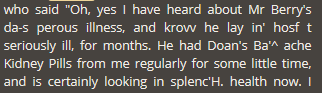
\includegraphics[width=9cm]{misspelling_1}
	\label{fig:misspelled}
	\caption{Text spelled poorly}
\end{figure}
%Should reference the testing reports again
%Discuss how my tests led to me narrowing the scope of the project down to information extraction and named entity recognition. 
%Feature actual test outcomes for the different software types used. 

\section{Database}
MySQL was used to build the database. Though SQLite was considered for a time it was felt that the use of a server would be required eventually, when taking into account the potential this system has to exist and grow into the future. SQLite was considered because it works well in low-memory environments and is easy to configure with no need for a server. At the current amount of information, SQLite would have been perfectly adequate, but would have severely limited the capabilities of the final system in other ways. DB-Engines Ranking\cite{db-ranking} ranks MySQL as the second most popular DBMS internationally and names it as being behind some of the largest websites and applications. On top of this,  it has extensive documentation and guides. It is fast and easy to use, and therefore was thought to be an excellent choice of database management system for this project. There was no discernable difference when comparing PostgreSQL to MySQL, so no reason PostgreSQL couldn't have been used instead. 

\section{Web App}

This system was initally planned around the use of Apache and PHP to build the web app. It is a series of tools that are commonly used, so are often standard for web development. After some problems using PHP to access data from the database, a different approach was considered using Flask.

Flask\ref{appendix:flask} is a web micro framework for Python that provides interfaces for other commonly used extensions. In this case, extensions used include \textit{SQLAlchemy} and \textit{wtforms}. After some brief experimentation, which involved setting up some basic HTML pages, and accessing them through a simple web app, it was felt that Flask would be a suitable framework to build with. The aim is also to host the app externally, so an investigation occurred into different options. Heroku and PythonAnywhere were the two webhosts considered: the former was almost immediately discounted as it does not offer native support for a MySQL database, and so time went into setting up using PythonAnywhere.

\chapter{Phase Two: Building the system}
This chapter focuses on the development of the system, looking at the three distinct parts; the information extraction, the storage of information, and how the information will be made accessible. Each section is broken down into the design, implementation and testing done for each section, as a lot of work done week to week builds upon each other, and there was no clear time period in which each section was worked on. This chapter covers from weeks three to approximately week ten though a lot of this work blurs into the work discussed in the previous chapter.
%This section pertains to developing the system around the experimentation code
\section{Information Extraction}
%Focus on back end code - extracting information into database
%What data I chose to extract
%Why I focused there instead of other areas
%Object Orientation and why

\subsection{Design}
The design of the system was built upon the experimentation discussed in the last chapter. As such, although the foundation for a larger system was already in place, the design and implementation occurred simultaneously. This made for some messy designs:
\begin{figure}
	\includegraphics[width=15cm]{IEflowchart}
	\caption{Information Extraction Flowchart}
	\label{fig:IEchart}
\end{figure}
%Insert data flow diagram and flowchart illustrating what I was trying to accomplish.
the flowchart shown in figure \ref{fig:IEchart} shows how the main method of the software works, task by task. All the data that this system can process starts out in a JSON file where, upon the starting of the program, the text of each article is extracted, and broken down again and again until the system is left with the information it is looking for: human names. For the time being, this and the article metadata is the only information considered important enough to be saved in the database.

Despite Python being an object orientated language, the inclusion of classes were not considered until much later into the project than they should have been. No class diagram has been produced because the classes serve little purpose outside of code readability and improving ease of maintenance.
%Still not sure if its worth a class diagram if my use of classes is so small.

\subsection{Implementation}
Before the process of information extraction could commence, the articles themselves had to be collected. The National Library of Wales has an API they provided access for the project, and with this a selection of articles could be saved to work with. To narrow the rather broad scope of `Science', five different fields were chosen to focus on: Astronomy, Biology, Chemistry, Mathematics and Physics. These were arbitrary choices, but it was felt that they would provide a good foundation upon which to build the system. There is no reason articles from, say, Psychology or Engineering could not be collected and processed in the same way. 

%this whole section probably needs rephrasing
The decision was also made to collect articles with a connection of some kind to one of these five fields and save the results in their own separate files, again for easy processing. The article collection code is kept separate from the information extraction, and the files stored locally because, due to the capabilities of the National Library servers, the API was only accessible to specific IP addresses. Setting up the collected data in such a way allowed development to continue without access to this API. This method of collection came with its own problems, but on the whole has worked well.
\begin{lstlisting}[caption={Information Collection}]
import requests	
import json

#p = "chemistry"
response = requests.get('http://papurapi.llgc.org.uk/?q=full_text\%3Aastronomy&fq=category
\%3A\%22News\%22&wt=json&indent=true&wt=json&indent=true&rows=999')
data = response.json()
file = open("astronomy.json", "w")
json.dump(data, file, sort_keys=True, indent=4)
file.close()
\end{lstlisting}
This is a very simple example of how the API can be used: it searches for 999 articles with the keyword \textit{Astronomy}, returns the results in JSON format and saves as a file. This method collected approximately 5000 articles with which to build a collection large enough for the purposes of this project. 

Once the articles had been collected, they had to be broken down into the information that was deemed important enough to extract: the newspaper title, the title of the article, the date upon which it was published, its unique identifying number, and the text that was printed in the article. This was all very simple to extract, because all of the information was already in JSON format, which Python can treat as a dictionary. The metadata that had to be sorted through to determine what was useful to the project was fairly extensive, though easily navigated. Figure \ref{fig:artmet} is an example of all of the available data about a single article.
\begin{figure}[h]
	\centerline{\includegraphics[width=20cm]{singleArticle}}
	\caption{Article Metadata}
	\label{fig:artmet}
\end{figure}
All of the information that is extracted from these files, with the exception of the article text itself, goes straight into creating a list of Article objects, which has four attributes and no class methods. This class was created to allow the attributes to be easily accessed for any particular article, which makes iterating over a list of these articles the easiest way to put compare them and put them in the database. A People class was also created for this precise reason.

It was mentioned in the previous chapter that some method of checking and correcting spelling would be useful to this project. This was done using a piece of code written by Peter Norvig\ref{appendix:norvig} that compares a word to a dictionary list of words, and generates the likelihood of a misspelled word being one or other of those words. It then attempts to correct the word to be the most likely alternative in two edit attempts. If it cannot, then the word stays misspelled. Without this code, it is unlikely that this software would be able to function properly, given the frequency with which spelling mistakes occur.

The key focus of this software is named entity recognition, which uses the NLTK \textit{ne\_chunk()} method to parse words into a shallow Tree structure. Its parameter is a list of part-of-speech tagged words. The chunk parser then looks at the tag attached to a word, and more specifically what the tag starts with. For certain tags, a tree will be built from that tag and its token, and then appended to the end of the larger, main tree. For other tags, they will be appended to the main tree as they are. This creates the shallow tree where child nodes that are not leaves are always entities. \cite{parser_documentation}
%Insert small example here of what the articles + metadata looks like
%Insert another example here of how the information is extracted.  

The task of determining the action from a newspaper article could have been approached in one of several ways. Building a classifier from the ground up was considered, and ultimately set aside as largely unnecessary; a similar result could be achieved using a list of potential 'actions', and searching through the text for any one of these. As with every other element of this project, the outcome from this approach would be less accurate than what a properly trained classifier could produce but would be suffice as a starting point.

Articles from all the different sciences considered for the system were read to decide what could constitute an action, and a few of the results are:
\begin{itemize}
\item Experiment
\item Lecture
\item Examination
\item Research
\end{itemize}
Though many articles were found to reference examination results of teenage and university students in the different sciences, these articles have been found to contain no information relevant to this collection. The \textit{Examination} keyword could be included to offer an easy method of filtering out irrelevant results. 

After all the important information has been extracted from the articles, a method of determining who is a scientist and who is not had to be implemented, since many articles mentioned upwards of a half dozen people each. The most obvious and accurate approach would have been building and training a classifier. There was, however, an easier method. Many articles were read, and how each one referred to its scientists was noted. People of note within newspaper articles are often referred to by their full name, and it appeared that scientists were no exception. Two lists of human first and surnames were compiled and, using the module \textit{HumanName Parser}\ref{appendix:humanName}, name objects were built from the named entities. The decision was made that only people who had a title, a first and a surname within the articles could be considered a scientist, as scientists would have been some of the more `respectable' members of society in the 1800's, and were therefore more likely to be referred to as such in newspapers. This method of recognizing scientists will inevitably pick up some people who are discussed within the articles and are otherwise people of notability, but this can be tweaked to omit results that exist within a different context based on the sentences they appear in. 

Three methods are shown below that work together to create people. First, a name is recognized to be real. A name could be considered `real' if it appears in either the list of first names or surnames. If both parts are considered real, then \textit{createName()} creates a HumanName object from these names. At this point, the name segments are in a list of tuples, where they were tokenized and tagged with the appropriate part of speech, so they must first be joined into a single string. Finally, once the name is made, the other attributes of the person can be set, the field of study and the article the person appeared in. 

\begin{lstlisting}[caption={Creating People}]
def createName(tuples):
	name_parts = []
	for tup in tuples:
		name_parts.append(tup[0])
		name = HumanName(' '.join(name_parts))
	return name
	
def isPersonReal(name):
		isReal = False
		with open("C:\backslash Users\backslash user\backslash Documents\backslash major_project\backslash what-made-scientists-in-wales-famous-and-infamous-1804-1919\backslash software\backslashtextfiles\backslash NAMES.txt", "r") as file:
			with open("C:\backslash Users\backslash user\backslash Documents\backslash major_project\backslash what-made-scientists-in-wales-famous-and-infamous-1804-1919\backslash software\backslash textfiles\backslash SURNAMES.txt", "r") as f:
				listOfNames = file.read()
				listOfSurnames = f.read()
				for names in listOfNames:
					if names[0] == name[0]:
					#if the first letter of the current name matches the first letter of the wanted name
					#makes the search through over 150000 names not take forever
						if name in listOfNames or name in listOfSurnames:
							isReal = True
						else:
							isReal = False
					else:
						continue
		return isReal
		
def createPeople(listOfPeople, fieldInt):
	lPeople = []
	for p in listOfPeople:
		names = p[0]
		aNumber = p[1]
		n = createName(names)
		if not str(n.first) == "" and not str(n.last) == "": #occassionally, a person had no first name. Index out of bounds error if not checked for.
			if isPersonReal(n.first) and isPersonReal(n.last) and not str(n.title) == "": 
				#if both names of the person are real names, and the person has a title
				study = fieldOfStudy[fieldInt] #fieldInt increased in the file for loop
				human = person.Person(n, study)
				#comment out the below line for testing purposes - Nothing in article_list
				#human.assignArticle(article_list[aNumber].id)
				lPeople.append(human)
		
	return lPeople
\end{lstlisting}

\subsection{Testing}
No user testing has been done on this part of the system, as the end user of the collection should not ever need to use it. The only job of the information extraction program is to look for information about scientists, and put that information into a database. The tests discussed in this section can be found in \textbackslash software\textbackslash information\_extraction of the project root directory, where they can be run any time any changes are made to the software. 

The test files discussed in this section have been created from five articles in each field of science, producing five smaller sets of data. This has been done to test new and edited methods in the software without waiting the literal hours it takes to search through a file of 999 articles.

\subsubsection{Unit Testing}
Unit testing was began early into the project timeline: as the need for more complicated methods grew, it was recognized that unit tests were the easiest way to ensure each part of the program ran exactly as expected. %Insert some description about what exactly was tested.
Initially writing the tests was harder than anticipated, due largely to a misunderstanding of the different data structures used in the NLTK pos tagging and named entity chunker. Some methods that did not end up used in the final program were also tested, primarily because it was evident at the time of implementation that these methods could serve a purpose to a developer later down the line, when additional information can be extracted. 
\begin{figure}[H]
	\centering
	\includegraphics[width=15cm]{error_textFindTest}
	\caption{findText() unit test error}
	\label{fig:ute1}
\end{figure}
Figure \ref{fig:ute1} shows a key error experienced when attempting to extract the full article text from one of the json files. The test behind this error found a bug where the same article would be written every time a new instance of \textit{``full text'': ``''} was found. This bug may have been missed completely until inspecting the entries in the database were it not for unit testing the method. 

A full report for the tests written can be found in appendix \ref{appendix:testSummary}.

\subsubsection{Integration Testing}
Unit integration testing, rather than system integration testing, then followed. This was designed to test how the different methods interacted with each other - it was noticed early into development that while expected outputs for methods were tested and determined to be properly functional in the unit testing portion of the testing phase, the types of these outputs were consistently confused when moving from method to method. For example, at the point \textit{createPeople()} is called, the input for this method is a list of tuples, where each tuple is itself a list of tuples. 

The interactions that were focused on in these tests are:
\begin{itemize}
	\item Text Collection
	\item Part of Speech tagging, Named Entity Recognition and the creation of scientists
	\item Repetition of information
	\item Interactions with the database
\end{itemize}
Though the final item in this list might be better suited to a system integration test, much of database manipulation relies upon several methods that also need to be tested for the proper interactions. This is why it has been included here. 

A full report for the tests written can be found in appendix \ref{appendix:testSummary}. However, an example has been included, to showcase how the format and assertion values were decided upon. 

The test in question, \textit{testTextCollection}, tests how the \textit{findText(), word\_tokenize()} and \textit{correctSpelling()} methods interact with each other. It was a logical choice to combine these methods into a single test, as their role in the program is to collect and manipulate an article's text. The code the test uses is identical to the code used in the program, with the exception that it has been isolated to make sense without the context of the rest of the program. Each method was run separately on a test file, which is essentially a scaled down version of a full file, and the resulting output from each method was manually inspected for expected output types and values. In the case of the \textit{correctSpelling()} method, an allowance had to be made for failed test: because this method uses probability, there is a fair chance that an assertion value that passes on one session of testing may fail on another. This is an issue with testing these kinds of methods, and does not reflect an issue in the code itself, nor in how it interacts with other methods. Finally, the output of the test was compared to the assertion list. A similar process was used to build the other unit integration tests. 
%Interactions for integration testing: put this in a document at some point
%FileA is read. JSON data is loaded
%findText() called
%LOOP: Article is read. Article is tokenized. Word is spellchecked. Word is tagged. Entites are tagged. PERSON entities are separated from tree. People are created. A person mentioned multiple times in a single article is removed. Articles are compared. If two articles are the same, one is removed from the article list. The scientist database is populated. The articles database is popuated. 

\section{Database}
%Includes focus on database design
%Include normalization process
%Include ER diagram
\subsection{Design}
The different kinds of information that a user could want to access was defined early in development:
\begin{itemize}
	\item Information about a scientist
	\item Information about a field of study
	\item Science by location
	\item The action a scientist may have performed to be in the paper
\end{itemize}
It was with these four potential queries in mind that the database was designed. 
\begin{figure}[H]
	\centering
	\includegraphics[width=9cm]{entity_relationship}
	\caption{Entity Relationship Diagram}
	\label{fig:er}
\end{figure}
The design of the database breaks down the above categories into three distinct parts; a scientist, an article and a newspaper. Figure \ref{fig:er} clearly indicates the relationship between these parts: an article cannot be part of more than one newspaper (this is in accordance with an article's unique identifier - during the period in history this project looks at, newspapers often offered a morning, afternoon and evening edition, where the same story could be printed multiple times.), but a newspaper is made up of multiple articles. An article could contain references to many scientists, or none, but a scientist must appear in at least one article. A scientist and article has several attributes that could be considered interesting enough to store in the database; the newspaper has only a title. The only reason the newspaper was considered to be interesting enough for the database is because, generally speaking, newspaper titles are a good indication of where the newspaper is published. Failing any specific location information within an article itself, it could at least be considered as being `from' the area of publication.


\subsection{Implementation}
Normalization in databases occurs because it increases the efficiency and accuracy of databases. Producing an example table based on figure \ref{fig:er} creates table \ref{table:1nf}. All of the article information for a single article is directly associated to a person, as are the name, date and location of the action they performed. There are three distinct pieces of information within a single table here which, apart from over complicating the database, could lead to a lot of unnecessary information being returned when a user searches for information. The full normalization process can be found in appendix \ref{appendix:normal}, but looking at table \ref{table:3nf}, it is evident that normalization was valuble to this database: the tables that were left after the process are more structured, and it will be easier to return specific results on behalf of the user compared to the initial table, despite that more tables often leads to longer query times.

\begin{table}[H]
\caption{Before Normalization}
\label{table:1nf}
\noindent\makebox[\textwidth]{
\begin{tabular}{|l|l|l|l|l|l|l|l|l|l|}
\hline
Name & Field & Action & Date & Location & News.Title & Art.Title & Art.Date & Contents & Art.ID \\ \hline
     &       &        &      &          &            &           &          &          &      \\ \hline
\end{tabular}
}%
\end{table}


\fbox{\begin{minipage}{27em}
\captionof{table}{After Normalization}
\label{table:3nf}
\begin{table}[H]
\begin{tabular}{|l|l|l|l|}
\hline
Scientist ID & Name & Field  \\ \hline
	& 		& 	 \\ \hline
\end{tabular}
\end{table}

\begin{table}[H]
\begin{tabular}{|l|l|l|l|}
\hline
Action ID & Action & Date & Location \\ \hline
	& 		& 		& \\ \hline
\end{tabular}
\end{table}

\begin{table}[H]
\begin{tabular}{|l|l|l|l|}
\hline
Newspaper Title & Article Title & Article Date & Article ID \\ \hline
                &               &              &            \\ \hline
\end{tabular}
\end{table}

\begin{table}[H]
\begin{tabular}{|l|l|l|}
\hline
Scientist ID & Article ID & Action ID \\ \hline
             &          &  \\ \hline
\end{tabular}
\end{table}
\end{minipage}}

The database was built using the MySQL workbench, which was chosen for no other reason that it was simple and quick to use. It was hosted on a server machine, which is the same machine that hosts the web server. This was the setup that the system was built and tested on, but for the final deployment, a server hosted externally should be  implemented, to ensure that the web app can function properly. This has the added benefit of being more secure than the test environment on a local machine that also hosts the web app: in the unfortunate event of a security breach of one server, the other would be independently protected. As the information stored in the database is designed to be accessed by the public, the only security risk pertaining to the database server that has been recognized is in the potential tampering with the information stored within it. 

\subsection{Testing}
The database, and the code that populated the database, was tested very simply using the same small data sets that the information extraction code was tested with. This was done because it allowed all testing to be performed at once, with each problem being identified as it popped up. A list of problems could be constructed from this, and worked on one by one until solved - this ensured that nothing was started then left incomplete. 

Although very little official testing was performed on the database, outside of that mentioned above, several issues were noticed with the information being stored. First, the assumption was made that all articles would have a title, and that titles would have a maximum length of around 50 characters. Neither of these cases were true, and the title field in the Articles table had to be adapted to accept null values for a title, as well as an increase in maximum length to well over a hundred characters. 

The database also required refilling several times, because there were several instances where the same article was found as belonging to multiple fields of study. This meant that there would be an attempt to store that article multiple times. Each article has a unique identifier, which is the primary key of the Articles table. There was more than one occasion where population of the database would stop because it was trying to store the same article ID multiple times. This was a problem with an easy fix, but was not found when testing with small samples because it was a rare enough occurrence that random selection of five or six articles from each field did not lead to it happening.

\section{Web App}
%Focus on design of web app
%Some CSS and HTML examples
%Talk about the problems with getting the app connected 
	%Compare initial apache and PHP trial vs FLASK route that I ultimately decided on
\subsection{Design}
The basic design of the web app was decided on fairly early into this project: appendix \ref{appendix:webUI} shows the initial design work as a simple search bar with a paragraph or two of written text describing what this project aims to accomplish, then subsequent pages show how a query would be returned. In the long term, the series of tables showing results feels a fairly simple way to display the information that has been collected, but it will suffice until such time as a more interesting display can be put together. 

The web app source code requires a redesign to improve readability and make it more maintainable. Several classes are currently housed in the same file; two classes that connect to tables in the database, and are extensions of SQLAlchemy's \textit{Model}, and one that creates a form for the homepage of the app. Because the app was produced with the aid of a Flask tutorial, it very quickly grew out of control. The following flowchart was produced alongside the app, in an attempt to better understand how the app needed to function.
\begin{figure}[H]
	\centering
	\includegraphics[width=17cm]{webAppFlowchart}
	\caption{Web App Flowchart}
	\label{fig:waf}
\end{figure}
It was with figure \ref{fig:waf} in mind that the app was built, with the primary purpose of acting as a search engine for the database. A secondary purpose was also considered: a reference to the article that the information came from in the first place. This was to take the form of a link to the article in the National Library of Wales archive, where the full thing could be read at the user's leisure.
%components of this system:
%Several classes that interface the database
%the HTML files
%the database
%the app itself

\subsection{Implementation}
The methods in the following section have been adapted from \url{https://www.blog.pythonlibrary.org/tag/flask/}
, which was used as a guide. Though the code is largely original, the basic premise is not.

The web app implementation began with a basic html page, that loaded with the start up of the app. This page, \textit{home.html}, offers a brief overview of what this project aims to achieve, along with a simple search form. The search form sends a query to the database, which returns a relevant list of results based on which kind of search was made as determined by the user via the drop down menu. The results are returned in a table, with a reference to the article that the searched information came from. This reference contains a hyperlink which takes the user to the National Library of Wales newspaper collection, to the article itself. These links were put together from the unique article ID.

\begin{lstlisting}[caption={Building URLs}]
	def returnLinks(resultsList, type):
	if type == 1:
		urls = dict()
		for result in resultsList:
			urlParts = re.split("-", result.articleID)
			url = '/'.join((urlParts[0], urlParts[2], urlParts[3]))
			urls[result.articleID] = url
	elif type == 2:
		urls = dict()
		for result in resultsList:
			urlParts = re.split("-", result.id)
			url = '/'.join((urlParts[0], urlParts[2], urlParts[3]))
			urls[result.id] = url
	return urls
\end{lstlisting}
In the above section of code, the \textit{type} determines what kind of search is being performed - one pertaining to a scientist, or an article. This difference is made in reference to the article ID for both: stored as the articleID in scientists, but id in articles. The URL parts shown above are sections of the id that create the url when reading an article on the archives. After breaking down the ID into parts by hyphens, only some of the parts are relevant, so those parts are then rebuilt into part of a url. Finally, the url-suffixes are returned as a dictionary of article IDs and the urls - it was believed at the time that this would make turning the results into a hyperlink easier. These can be attached to the url root, which is the same for every article.

Once the query results have been returned, the next step is to put the results in a table and display the table. Two \textit{tables} classes were built using flask\_table, one for scientists and one for articles, which displayed different results depending on the 
type of search made. These tables, now filled with the query results, are sent to the \textit{results.html} file, which displays the results. 

A key area of difficulty was in deciding how to host the web app. One of the final decisions made for this project was in deciding whether to host the app locally for the project life span, which would be the simpler but less professional option, or in attempting to host externally. The latter option had the added benefit of  being accessable from anywhere at any time, which is a vital part of any application designed around use by a larger group. The app was not built with external hosting in mind, so setting up the system to be hosted externally was difficult. In particular, because this app should be accessible from anywhere at any time, the MySQL database had to be hosted externally as well, which meant filling another database. As of the writing of this report, the app still cannot be hosted externally, though it is still an aim of the project and this feature is still in development. 

\subsection{Testing}
As detailed in appendix \ref{appendix:testSummary}, the website was tested to ensure that different searches return different results that match the search. The same set of search terms were used for each category of search:
\begin{itemize}
	\item The name \textit{Robert Smith}.
	\item A partial search based on the name above, \textit{Smi}.
	\item The field \textit{Chemistry}.
	\item Part of an article title, \textit{Professor Mag}.
	\item A full article title, \textit{Death of Professor Magnus}.
\end{itemize}
These tests passed, and helped make the app easier to use in determining that some method of informing the user that their search was invalid would make their experience using the web app more pleasant. Some of the tests in the testing summary allude to the implementation of other features outside of those already discussed in this report as being useful to a user: in particular, a method of filtering results that have already been found would help navigate those searches that lead to many search results from many different fields, such as searching for an article title.

Manual testing was also useful in determining where the issues with the hyperlinks back to the National Library archive lay: through a series of print statements and trial and error, it was determined that the issue is not with building the URL themselves, nor with redirecting a user to the web page, as both of these features work separately. The issue is in connecting the URL to an individual article ID, and doing this for each article. It is suspected that this issue comes from inexperience in using Flask.

\chapter{Evaluation}
This chapter discusses an overall evaluation of the project. It includes how I utilized my chosen methodology to its full potential, the work actually completed in the time frame, and my own understanding of the project. 
%Chapter on what went well, and where I fucked up. 
\section{What I have learned}
Before starting this project, I knew nothing about natural language programming. I'd never heard of it, let alone considered what it's applications might be or how it could be implemented. In order to complete this piece of work, I had to learn how language works; what different parts of speech were and what they were for, what an entity was and how it differed to a named entity. I also needed to understand what natural language could be used for, that I knew what techniques would be useful to apply to this project and what would not. Towards that end, I turned to web articles designed as a casual introduction into NLP.

Though I had done some work in Python previously, this was my first major piece of work in the language. I suspect that led to me making many mistakes, namely in not utilizing classes until far later in the project than I should have, in writing inefficient code and taking far longer in writing tests than was reasonable. Despite the issues I have had using Python, I do not regret its use as the primary language for the system: I suspect there would have been far more issues had I used Java or C++. 

This project introduced a lot of firsts for me: NLP, working with an API, automating database population, using Flask and SQLAlchemy, and using Python's UnitTest. 

Flask was particularly difficult to really use properly, despite following a tutorial for most of it, as I didn't understand why I was writing the code that I was until a week or two later. This made it difficult to know where bugs were coming from and, I suspect, is a contributing factor to why the final web app feels underwhelming. In future, I may just stick to a tutorial to provide an introduction to a technology, and use its documentation as the primary source of assistance.

The Python Unittest module proved really easy to use. I did not focus as much on learning what the module was capable of, preferring to only learn what I needed to get by. This is evident in the way every unit test, and even the integration tests, are implemented in exactly the same way. 

\section{On the Chosen Methodology}
As described in Chapter One, the chosen methodology for this project was scrum, with some kanban elements where needed. Kanban did not prove as useful to managing the system's workload as was initially expected and was soon cast aside in favour of a more traditional scrum based system. This was the right decision, as the weekly iterations provided invaluable flexibility to the project organization, without which this system might never have been built to its current level of completion. The amount of work aimed for each week was often severely underestimated to the point where, after the weekly sprint meeting every Monday morning, the work prioritised for that week would be finished by Wednesday or Thursday. This led to an adjustment in how each iteration was organised. Early sprints focused on a single task and its design, implementation and testing, but it was quickly realised to be an inefficient way to work: although a deeper look into any particular feature could not be done until the next iteration, an entirely independent aspect of the system could also be designed, implemented and tested. Had this adjustment taken place sooner in the project timeline, instead of a fixation on finishing one aspect or element of the system, then there may have been more time to implement more features, and the system may have ended up looking and feeling a lot more refined to use. 

\section{Deviations from the Plan}
Due to poor time management, emphasis was placed on implementing functional requirements as best as possible, at the cost of not implementing them all. Therefore, while the system can allow for several different searches, it cannot handle dealing with multiple queries at once. While there is the infrastructure to provide a reference link to where a specific article came from, the actual implementation does not work. It was also sorely overestimated how much information on any one scientist would be available from newspapers alone, which meant functional requirement \textit{1.4: Summarize the information about a specific person in cases where a specific name is returned or searched for} was not feasible within the constraints of this project. 

A key aspect that was to be implemented was finding and extracting what scientists did to end up in newspapers: in the beginning of the project, I had hoped to build this into the collection to show some of the ways in which Welsh people contributed to the scientific advancements of the age. It could also have been used to make the collection more interesting to a wider audience; a collection showing scientists in negative ways, as criminals, as chemists accidentally causing fires or explosions, as being the kinds of people who could do anything they wanted simply to see what would happen, could be a collection that excites the minds and imagination of young people, for whom science, particularly that long ago, can seem stuffy and dull. Unfortunately, this was not a feature that I could implement within the constraints of the project: I got so focused on producing a working system, and invested so much time into learning new tools and technologies, that there wasn't enough to devote to this part. I truly regret not working on this feature, and if I have the chance to continue work on this project, it is something I will prioritize. 

\bibliographystyle{ieeetr}
\bibliography{finalReport}

\appendix
\chapter{Third Party Code and Libraries}

\section{NLTK}
\label{appendix:nltk}
\color{blue}[1]\color{black}:\url{http://www.nltk.org/}\\
This is the toolkit that the whole project depends on. It provided the tools needed to break down the articles and extract the required information from them. The NLTK is licensed under the Apache License V2.0.

\section{Spell Corrector}
\label{appendix:norvig}
\color{blue}[2]\color{black}: \url{http://norvig.com/spell-correct.html}\\
Code from this website was used to correct spelling mistakes in articles that were vital for proper information extraction, without which this project wouldn't have been half as successful as it is. At the time of writing, the website above seems to be inaccessible, but is the same as the one used originally. The same code can also be accessed here: https://github.com/norvig/pytudes/blob/master/py/spell.py
This code is licensed under the MIT licence. An edit was made to the code to allow for a third iteration of searching for potential corrections: though this was ultimately not used for this project, it has been left in the source code in case it becomes necessary for future development.

\section{Spell Checking}
\label{appendix:spellchecker}
\color{blue}[3]\color{black}: \url{https://stackoverflow.com/questions/40188226/nltks-spell-checker-is-not-working-correctly}\\
Code here was used to implement a checker for whether or not a word is misspelled. This was used to prevent the spell checker searching every single word in every single article for misspellings. Code on stack overflow falls under the Creative Commons BY-SA 4.0 license \textit{\url{https://creativecommons.org/licenses/by-sa/4.0/}}.

\section{Human Name Parser}
\label{appendix:humanName}
\color{blue}[4]\color{black}: \url{https://nameparser.readthedocs.io/en/latest/}\\
This module was used to build human name objects from strings, simplifying the process of determining whether or not a person was real and, if they were real, whether or not they were a scientist. This module is available for use under the LGPL-2.1 license.

\section{Flask}
\label{appendix:flask}
\color{blue}[5]\color{black}\url{http://flask.pocoo.org/}\\
Flask was the framework used for the web app. It is licensed under a BSD license: \url{http://flask.pocoo.org/docs/1.0/license/}\\
Flask interfaces used in this project are \textit{flask\_sqlalchemy} to connect with SQLAlchemy and \textit{flask\_wtf} with FlaskForm.

\chapter{Ethics Form}

\includepdf{ethics_form.pdf}

\chapter{External Documents}
\section{Requirements}
\label{appendix:requirements}
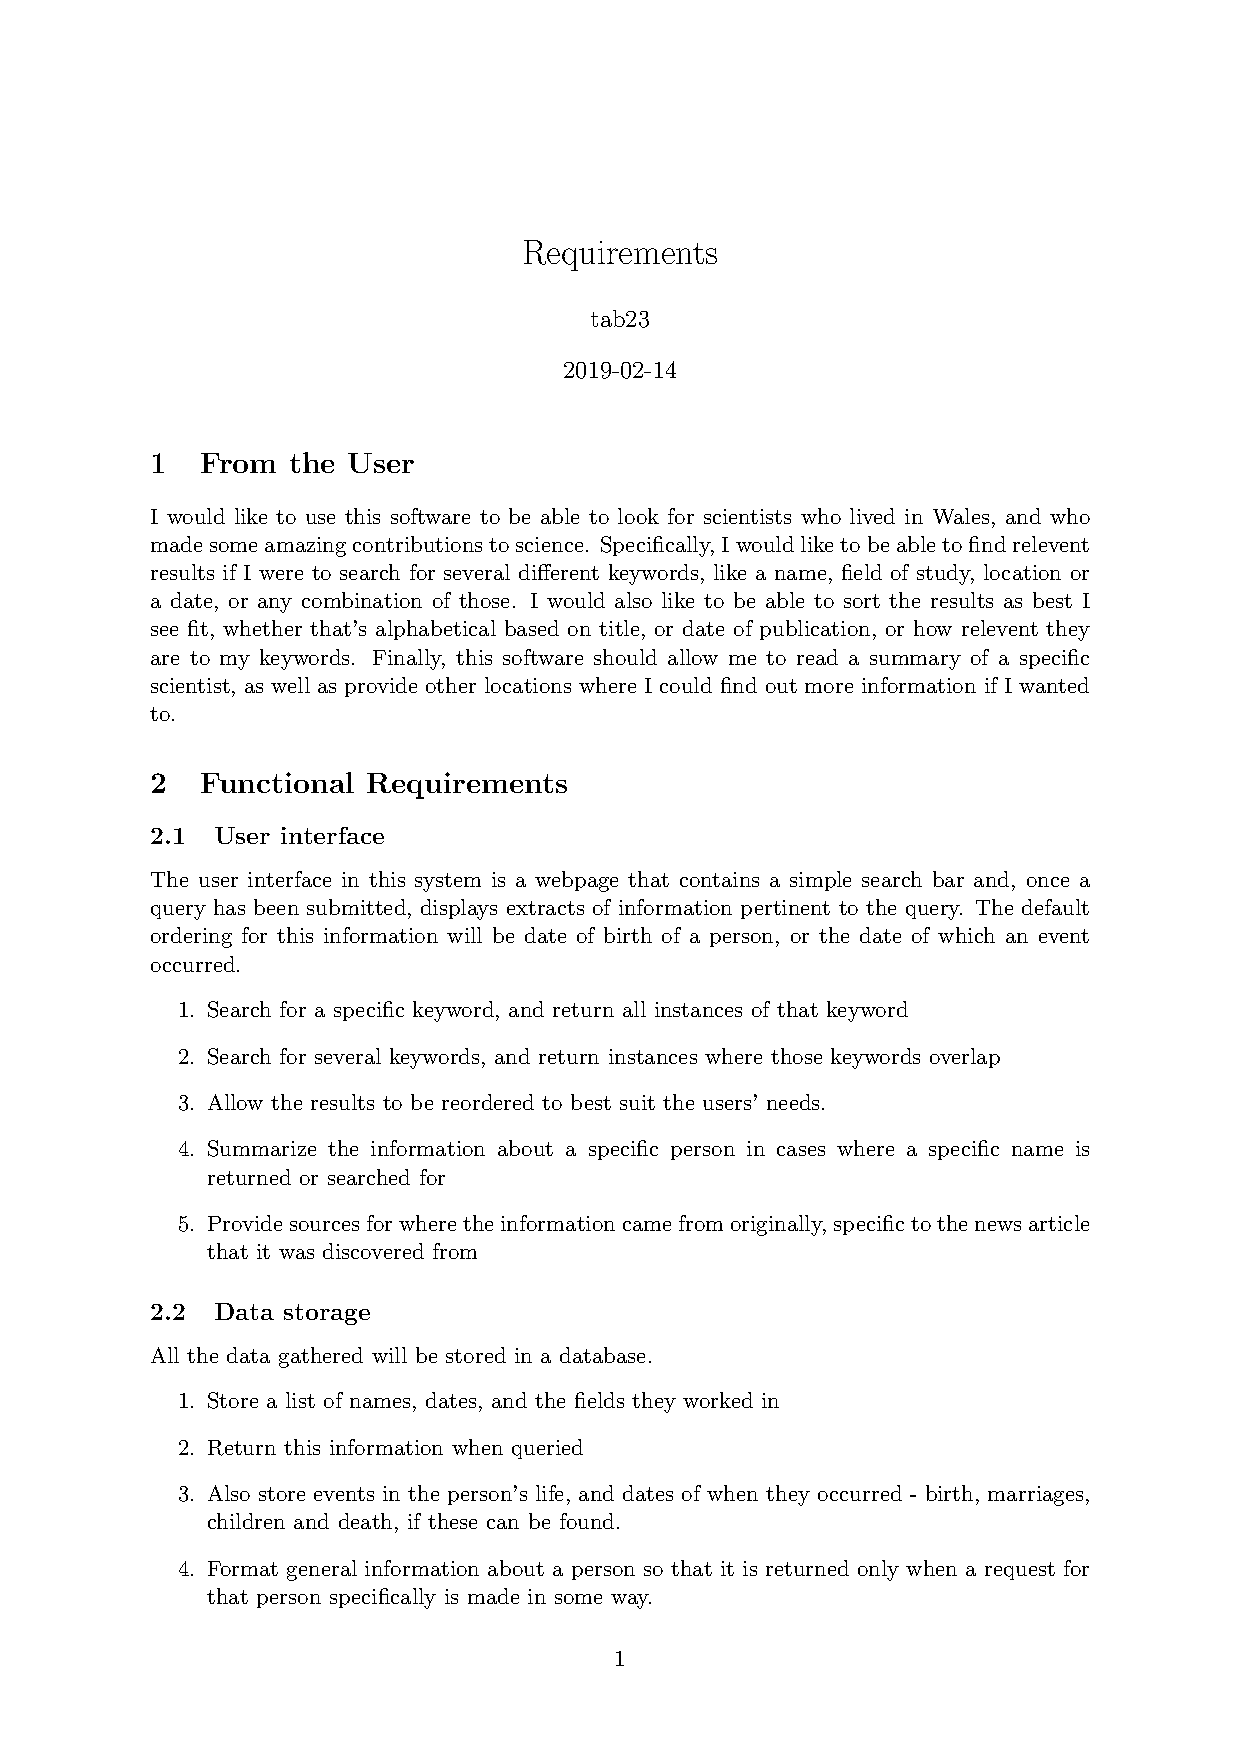
\includepdf[pages=-]{requirements.pdf}
\section{NLP Toolkit Comparison}
\label{appendix:comparison}
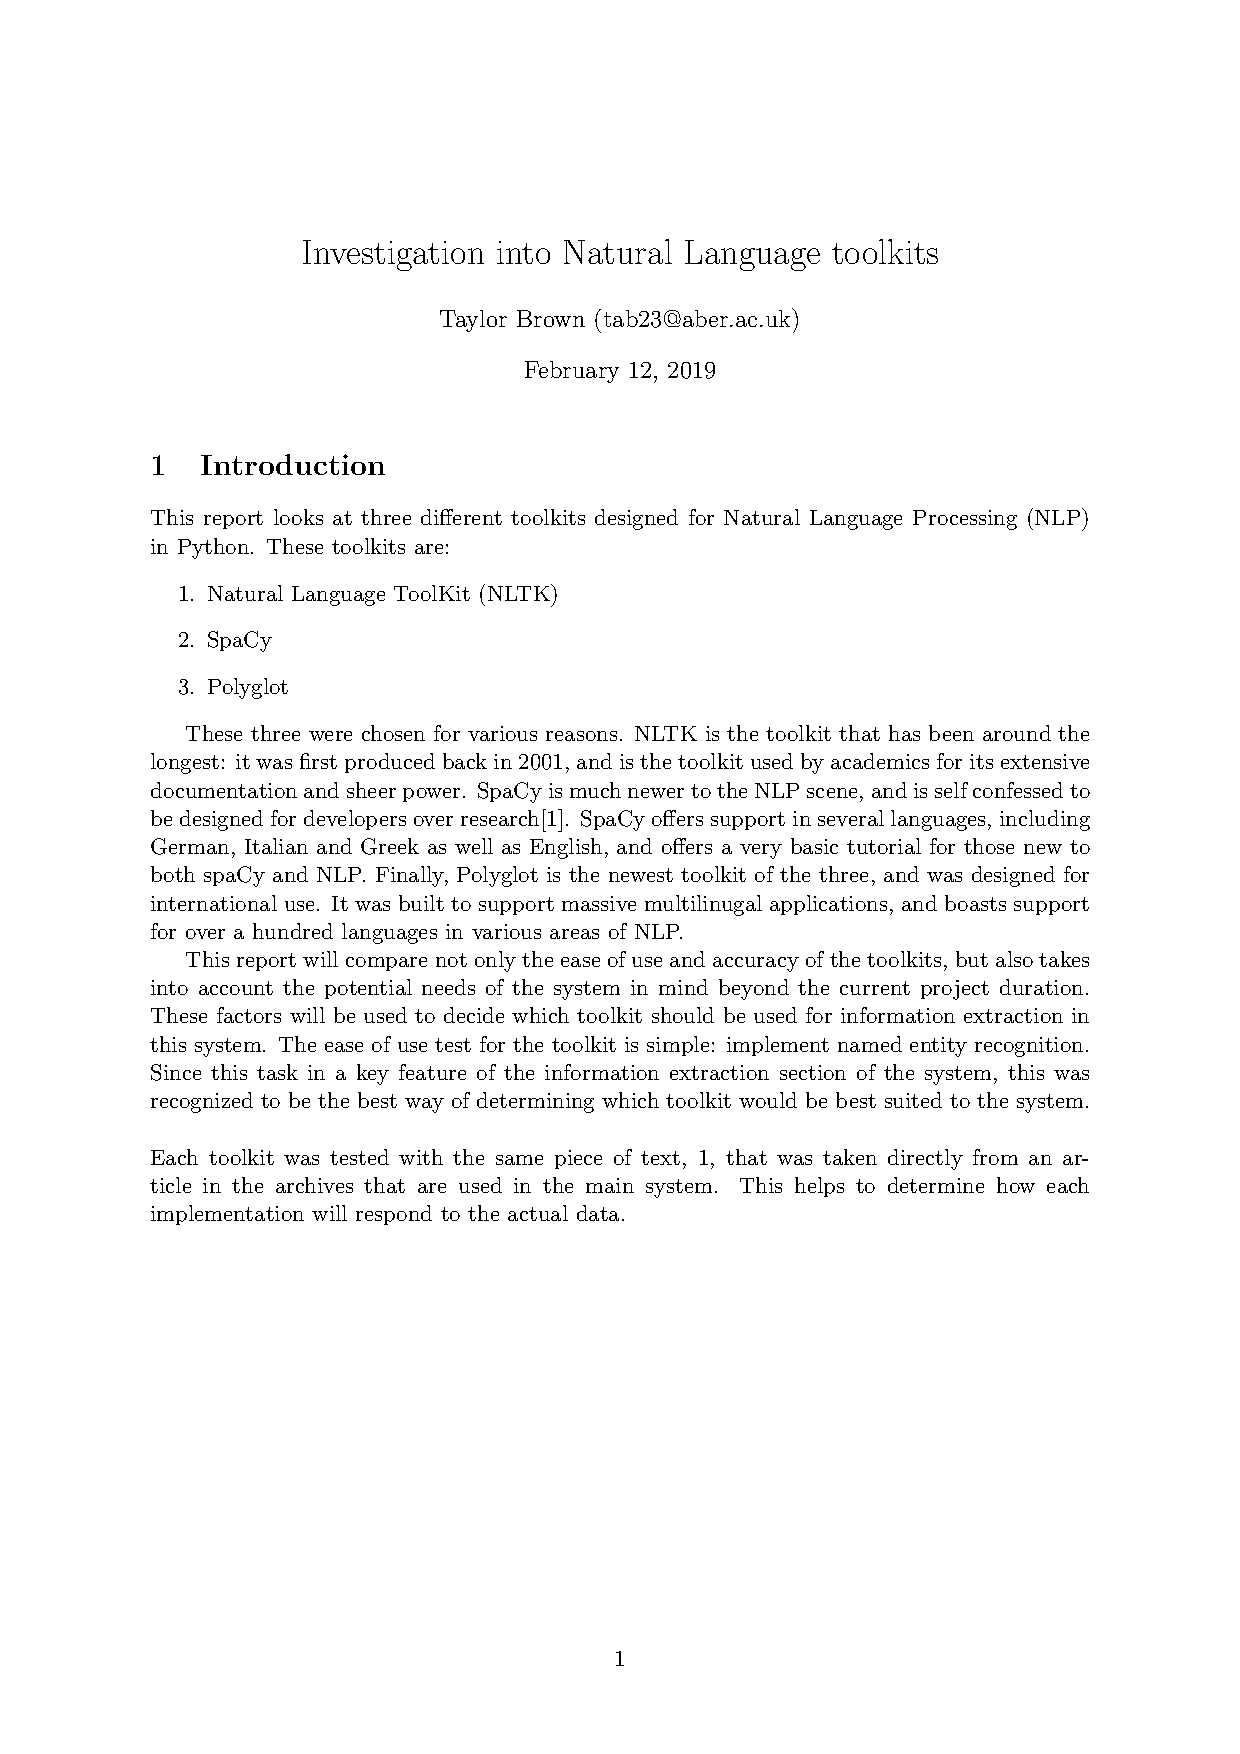
\includepdf[pages=-]{NLPtestingReport.pdf}
\section{Database normalization}
\label{appendix:normal}
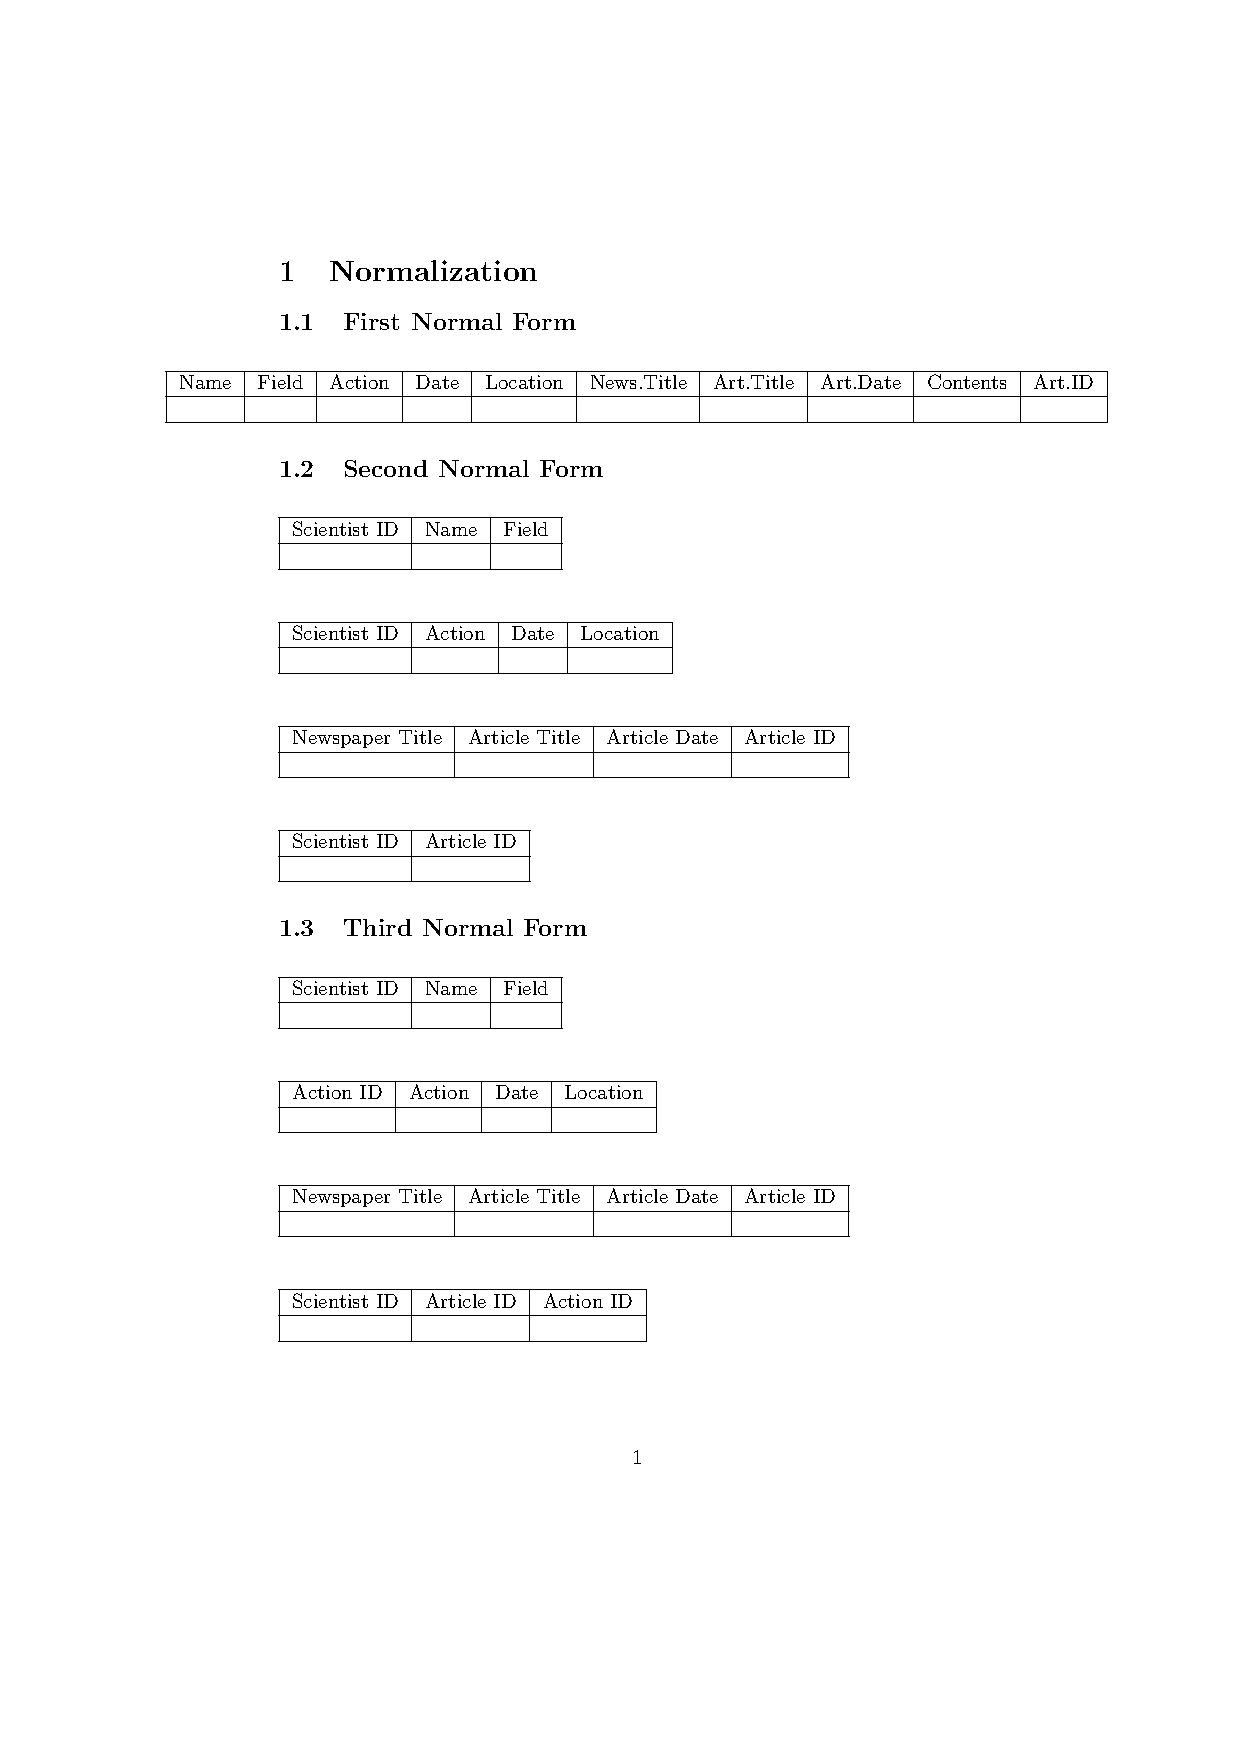
\includepdf[pages=-]{table_normalization.pdf}
\section{Testing Summary}
\label{appendix:testSummary}
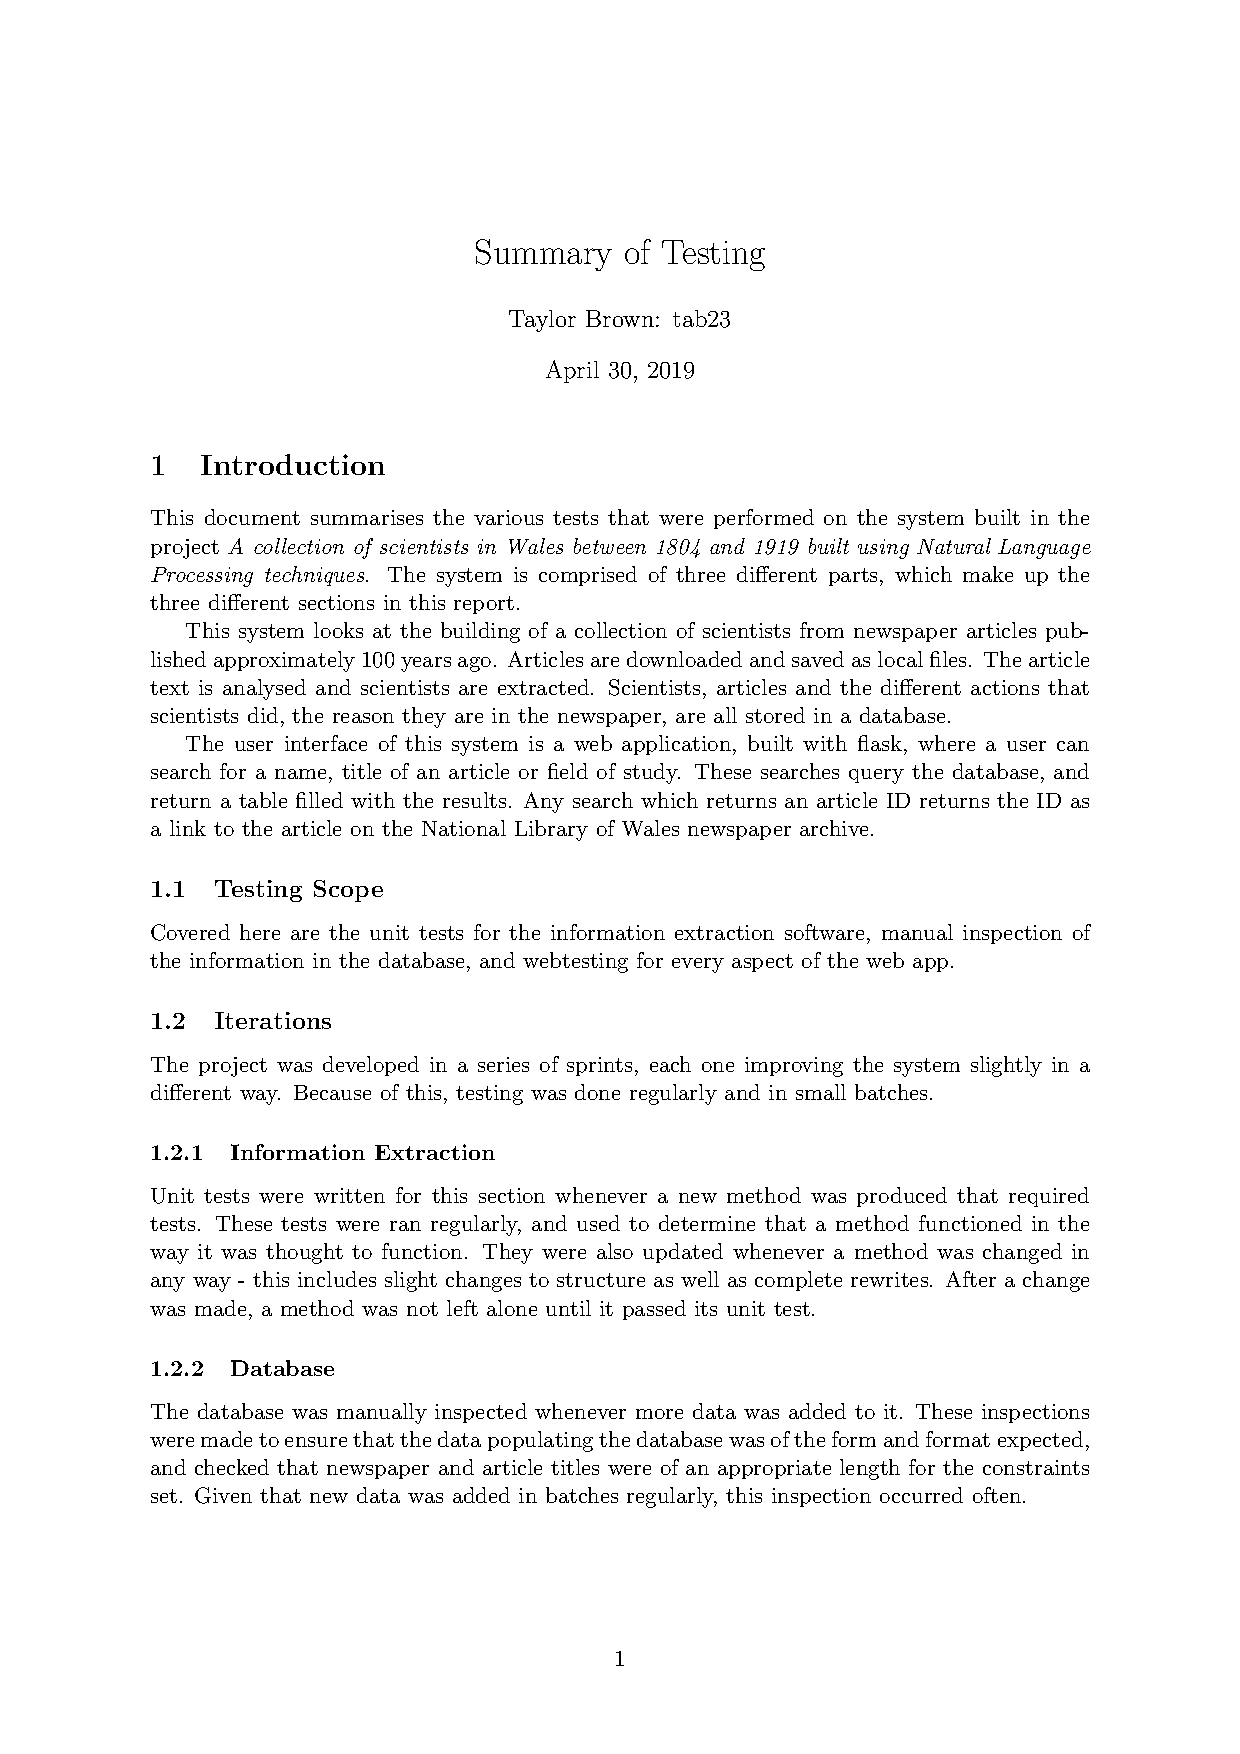
\includepdf[pages=-]{testingSummary.pdf}
\section{Web Application Design}
\label{appendix:webUI}
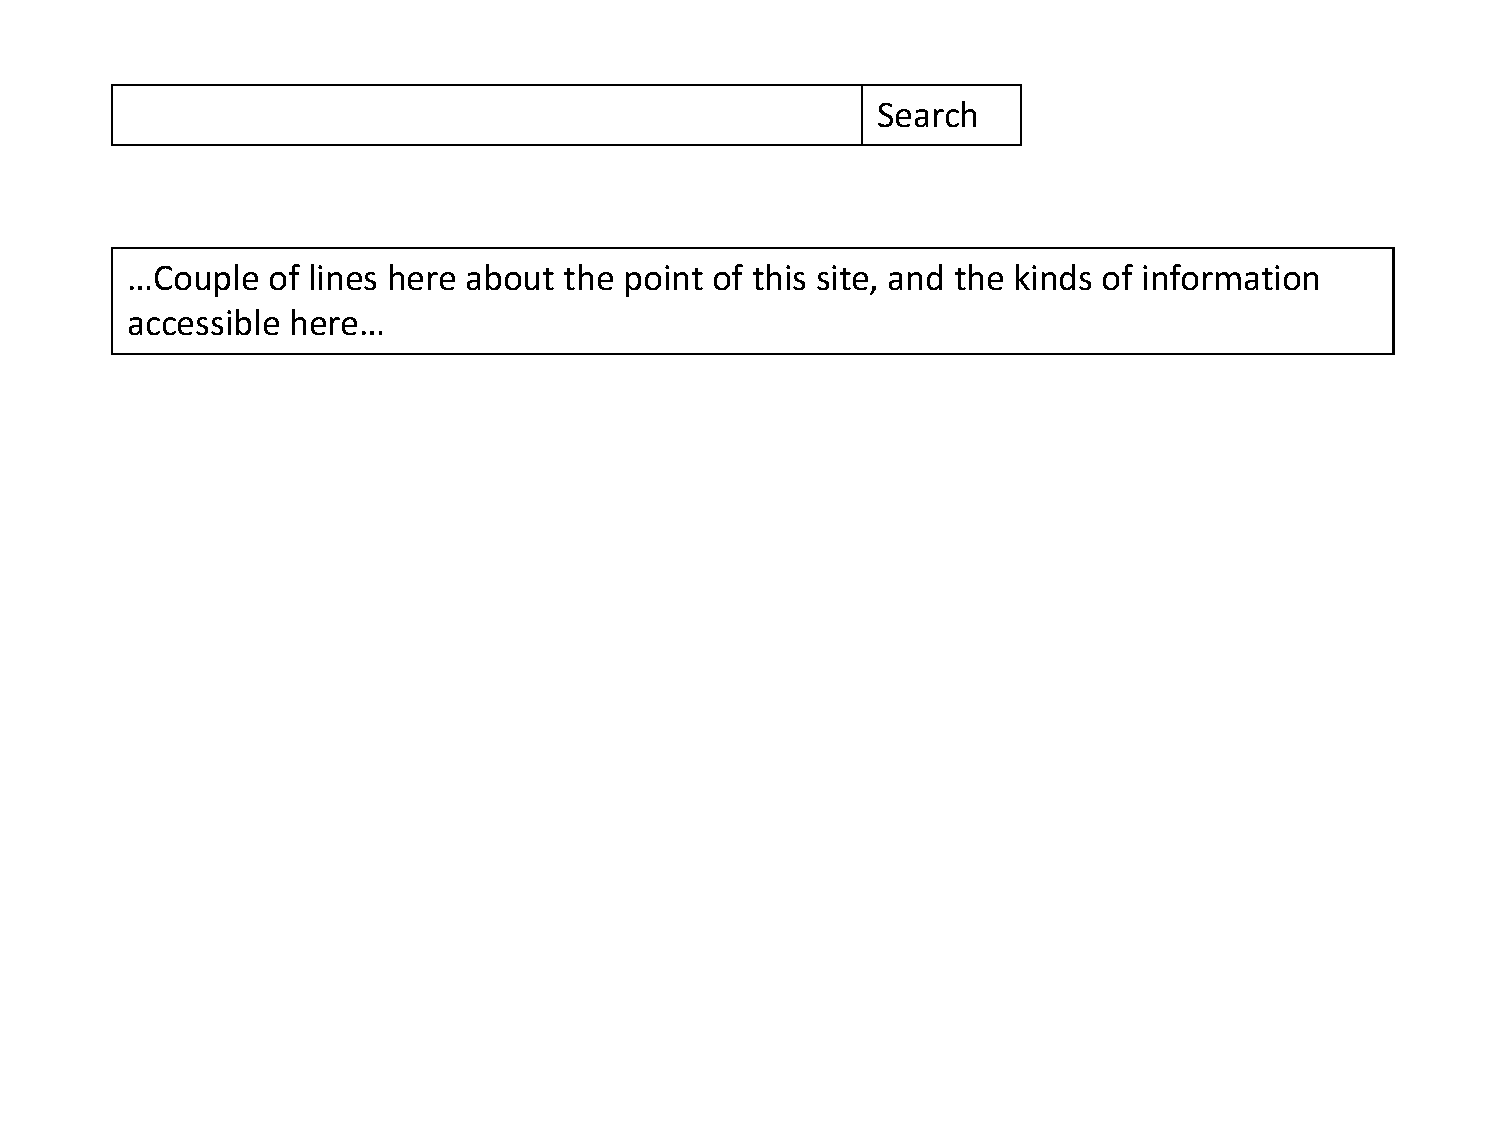
\includepdf[pages=-]{web_ui.pdf}

\end{document}